\section{Introduction}

%****************New Frame******************
\begin{frame}[c]{Why is online adaptation needed?}
    Being the ultimate goal to better conform dose to the target\ldots
    \begin{itemize}
        \item<1-> \textbf{Setup} uncertainties
        \item<1-> Patient \textbf{anatomy} inter-fractional variation
        \item<2-> Protons are sensitive to geometry changes
        \item<2-> Target \textbf{coverage} may be compromised
        \item<3-> Security \textbf{margins} increase high dose region
        \item<4-> Higher dose to \textbf{OARs}
        \item<5-> A risky statement: \textbf{Robust planning} can not cover every possible scenario and increases high dose volume
    \end{itemize}
    \onslide<6->{
        \begin{exampleblock}{}
            Online adaptation would allow margin reduction guaranteeing coverage and OAR sparing at before every fraction is delivered
        \end{exampleblock}
    }
\end{frame}


\begin{frame}[c]{The Head and Neck case}
    \begin{columns}[c]
        \begin{column}[c]{0.45\textwidth}
            \begin{figure}[h]
                \centering
                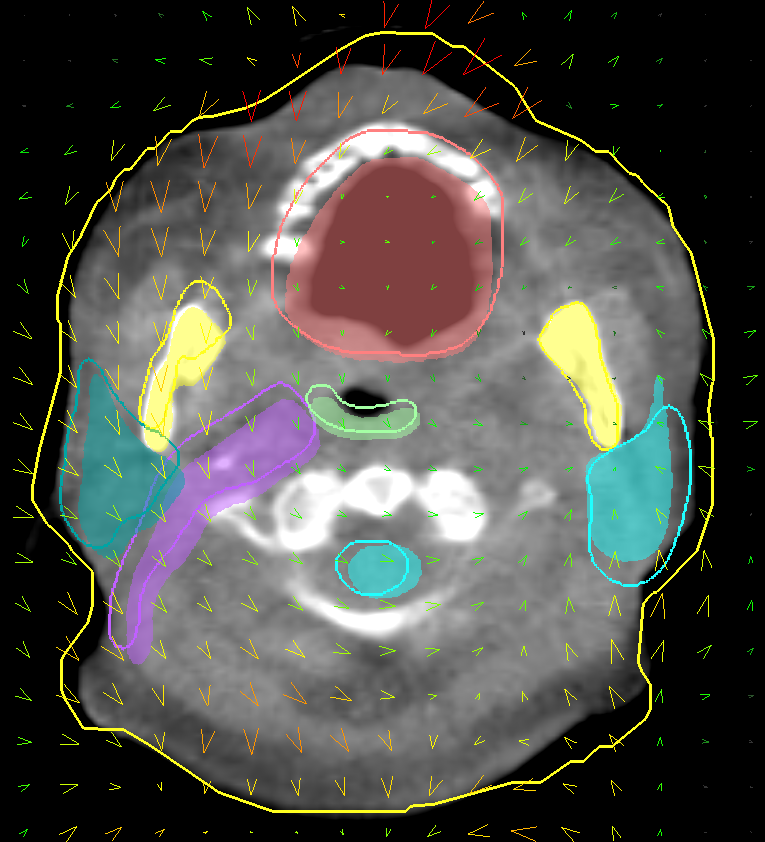
\includegraphics[width=\textwidth]{imgs/patient_deformation.png}
                \caption{Head and neck patient geometry changes. The arrows represent the vector field.}
            \end{figure}
        \end{column}
        \begin{column}{0.55\textwidth}
            \textbf{Potential for increased treatment quality:}
            \begin{itemize}
                \item OARs very close to the target
                \item Large inter-fractional anatomy changes
                \item Tissue interfaces make it sensitive
            \end{itemize}
        \end{column}
    \end{columns}
\end{frame}

\section{Objectives}
\begin{frame}[c]{Objectives:}
	Aim: Change the IMPT fields to recover initial plan quality while the patient is on the couch
	
    Goals:
    \begin{itemize}
    	\item Develop an \textbf{online} adaptation algorithm
    	\item Dose calculations with GPU-MC on CBCTs
    \end{itemize}
    \pause
    Steps:
    \begin{itemize}
        \item Plan set of patients with IMPT and no margin on CTV
        \item Study plan evolution \textit{vs} anatomy changes on CBCT images
        \item Can we get away with plan adjustments as opposed to replanning?
    \end{itemize}
\end{frame}

\begin{frame}[c]{What has been published?}
	\begin{columns}[c]
		\column{0.5\textwidth}
		\begin{block}{Kurz 2016}
			\begin{itemize}
				\item Offline
				\item Analytical dose calculation
				\item Full reoptimization
				\item Adaptation on vCT
			\end{itemize}
		\end{block}
		\begin{block}{Moriya 2017}
			\begin{itemize}
				\item Range shifter of the day
				\item Passive scattering for lung
			\end{itemize}
		\end{block}
		\column{0.5\textwidth}
		\begin{block}{Jagt 2017}
			\begin{itemize}
				\item Online (more or less)
				\item Analytical dose calculation
				\item Dose restoration
				\item Full reoptimization
				\item Original contours
			\end{itemize}
		\end{block}
		\begin{block}{Bernatowitz 2018}
			\begin{itemize}
				\item Extension of \textit{Jagt et al.} for robust optimization and others
			\end{itemize}
		\end{block}
	\end{columns}
\end{frame}




